%<dscrpt>Introduction à la programation linéaire</dscrpt>
Ce texte\footnote{d'après \emph{Combinatorial Optimization.}; C. H. Papadimitriou , K Steigliz; Dover} introduit l'algorithme du simplexe. Il s'agit de minimiser une fonction coût dans un ensemble convexe de solutions d'un système d'équations et d'inéquations.
\begin{quote}\textit{
  La partie 0 ne contient pas de questions mais rassemble toutes les notations. Il est conseillé de la lire une première fois sans chercher à tout mémoriser puis d'y revenir pour trouver ce que représente une notation rencontrée plus loin.}
\end{quote}
\subsection*{Partie 0. Notations}
\noindent
Soit $m$ et $n$ entiers avec $0 < m < n$.
\subsubsection*{1. Formes linéaires de $\R^n$}\noindent
La base canonique de $\R^n$ est notée $\mathcal{E} = (e_1,\cdots,e_n)$. On rappelle que
\[
  \forall j \in \llbracket 1,n \rrbracket, \;
  e_j = (0, \cdots, 0, \underset{\text{indice }j}{\underbrace{1}},0, \cdots, 0).
\]
Soit $(\alpha_1, \cdots , \alpha_m)$ une famille de formes linéaires de $\R^n$ dans $\R$. On note
\[
  \forall i \in \llbracket 1, m \rrbracket,\, \forall j \in \llbracket 1, n\rrbracket:\: a_{i j} = \alpha_i(e_j).
\]
Les $a_{i j}$ définissent une matrice $A \in \mathcal{M}_{m n}(\R)$. On introduit aussi l'intersection des noyaux
\[
   S = \ker \alpha_1 \cap \cdots \cap \ker \alpha_m .
\]
On introduit une autre forme linéaire notée $\gamma$ de $\R^n$ dans $\R$. Elle est appelée \emph{forme (ou fonction) coût}.\newline
On note $c_j = \gamma(e_j)$ pour tous $j \in \llbracket 1,n \rrbracket$ et \textbf{on suppose} $\forall j \in \llbracket 1,n \rrbracket,\; c_j >0$.

\subsubsection*{2. Matrices colonnes}\noindent
Dans $\mathcal{M}_{m 1}(\R)$ (le $\R$-espace vectoriel des matrices colonnes à $m$ lignes), on note
\[
  \forall j \in \llbracket 1, n\rrbracket,\; v_j = C_j(A)
  =
  \begin{pmatrix}
    a_{1 j} \\ a_{2 j} \\ \vdots \\ a_{m j}
  \end{pmatrix}\; \text{ et }
  b=
  \begin{pmatrix}
    b_1 \\ b_2 \\ \vdots\\ b_m
  \end{pmatrix}
.
\]
\textbf{On suppose que $(v_1, \cdots, v_n)$ engendre $\mathcal{M}_{m 1}(\R)$ et que $b\neq 0_{\mathcal{M}_{m 1}(\R)}$ .}\newline
On note $\mathcal{X} = (X_1, \cdots ,X_m)$ la base canonique de l'espace $\mathcal{M}_{m 1}(\R)$ des matrices colonnes.

\subsubsection*{3. \'Equations}\noindent
On s'intéresse au système d'équations d'inconnue $x = (x_1, \cdots, x_n)\in \R^n$:
\[
  \left\lbrace
  \begin{aligned}
    \alpha_1(x) &= b_1\\
    \alpha_2(x) &= b_2\\
    \vdots \\
    \alpha_m(x) &= b_m
  \end{aligned}
  \right.
\Leftrightarrow 
A 
\begin{pmatrix}
  x_1 \\x_2 \\ x_3 \\ \vdots \\ x_{n-1} \\x_n
\end{pmatrix}
= b.
\]
On note $\mathcal{S}$ l'ensemble des solutions de ce système. Par définition $\mathcal{S} \subset \R^n$.\newline 
On remarque que $S = \ker \alpha_1 \cap \cdots \cap \ker \alpha_m$ est l'ensemble des solutions du système homogène
\[
  \forall i \in \llbracket 1,m \rrbracket, \; \alpha_i(x) = 0.
\]
On note $\mathcal{S}^+ = \mathcal{S} \cap (\R^+)^n$ l'ensemble des solutions \emph{positives}:
\[
  \forall x = (x_1, \cdots, x_n) \in \R^n,\;
  x \in \mathcal{S}^+ \Leftrightarrow
  \left\lbrace
  \begin{aligned}
    \forall i \in \llbracket 1, m\rrbracket &, \alpha_i(x) = b_1\\
    \forall j \in \llbracket 1,n \rrbracket &, x_j \geq 0
  \end{aligned}
  \right. .
\]
Les éléments de $\mathcal{S}^+$ sont appelés des solutions \emph{acceptables}.\newline
\textbf{On suppose que $\mathcal{S}^+ $ est non vide.}

\subsubsection*{4. Ensembles d'indices}\noindent
Pour tout $z = (z_1, \cdots, z_n) \in \R^n$, on introduit des notations liées aux signes des valeurs:
\[
\begin{aligned}
  &J^+(z) = \left\lbrace j \in \llbracket 1 ,n \rrbracket \text{ tq } z_j > 0\right\rbrace, \; n^+(z) = \card (J^+(z))\\ 
  &J^-(z) = \left\lbrace j \in \llbracket 1 ,n \rrbracket \text{ tq } z_j < 0\right\rbrace, \; n^-(z) = \card (J^-(z))\\
  &J(z) = \left\lbrace j \in \llbracket 1 ,n \rrbracket \text{ tq } z_j \neq 0\right\rbrace = J^+(z) \cup J^-(z)\\
  &n(z) = \card (J(z)) = n^+(z) + n^-(z).
\end{aligned}
\]
Ces ensembles d'indices (parties de $\llbracket 1,n \rrbracket$) seront utilisées pour des solutions $x\in \mathcal{S}$ et pour des vecteurs $u\in S$ dans l'intersection des noyaux.\newline
Pour toute partie $J$ de $\unAn$, on note $\overline{J} = \unAn \setminus J$. Par exemple 
\[
  \overline{J(x)} = \left\lbrace j \in \unAn \text{ tq } x_j = 0\right\rbrace.
\]

\newpage
\subsection*{Partie 1. Questions de cours}
\begin{enumerate}
  \item Questions de rangs.
  \begin{enumerate}
    \item Soit $i \in \llbracket 1,m \rrbracket$ et $x=(x_1, \cdots, x_n)$. Exprimer $\alpha_i(x)$. Préciser $\Mat_{\mathcal{E} (1)}(\alpha_i)$ où $(1)$ désigne la base de $\R$ considéré comme un $\R$-espace vectoriel.
    \item Rappeler la définition du rang des lignes de $A$, la définition du rang des colonnes de $A$, la proposition liant ces deux notions et le principe de sa démonstration. 
    \item Montrer que $\rg(A) = m$ et que $(\alpha_1,\cdots, \alpha_m)$ est libre dans $\mathcal{L}(\R^n,\R)$.
  \end{enumerate}
  \item Dimension de $S$.
  \begin{enumerate}
    \item Justifier que l'on peut compléter $(\alpha_1, \cdots, \alpha_m)$ en une base $(\alpha_1, \cdots, \alpha_n)$ de $(\R^n)^*$.
    \item Montrer que $\ker(\alpha_1) \cap \cdots \cap \ker(\alpha_n) = \left\lbrace 0_{\R^n} \right\rbrace$. On pourra considérer les applications
\[
  \forall j \in \llbracket 1,n \rrbracket, \;
  \left\lbrace
  \begin{aligned}
    \R^n &\rightarrow \R \\ 
    (x_1, \cdots, x_n) &\mapsto x_j
  \end{aligned} \right. .
\]
   \item On définit des applications $\Phi$ et $\Psi$:
\[
  \Phi :
  \left\lbrace
  \begin{aligned}
    \R^n &\rightarrow \R^n \\
    x &\mapsto (\alpha_1(x), \cdots, \alpha_n(x))
  \end{aligned}
   \right., \hspace{0.5cm}
     \Psi :
  \left\lbrace
  \begin{aligned}
    \R^n &\rightarrow \R^m \\
    x &\mapsto (\alpha_1(x), \cdots, \alpha_m(x))
  \end{aligned}
   \right. .
\]
Montrer qu'elles sont surjectives. En déduire $\dim S = n -m$.
  \end{enumerate}

  \item Solutions.
  \begin{enumerate}
    \item Montrer que $\mathcal{S} \cap S = \emptyset$ et que $\gamma(x) >0$ pour tout $x\in \mathcal{S}^+$.
    \item Soit $x_0 \in \mathcal{S}$. Montrer que $\forall x\in \R^n, \; x \in \mathcal{S} \Leftrightarrow x- x_0 \in S$.\newline
On dit que $\mathcal{S}$ est un sous-espace affine de $\R^n$ de direction $S$.
    \item Montrer que $\forall (x,y) \in {\mathcal{S}^+}^2, \forall \lambda \in \left[ 0, 1 \right]:\; \lambda x + (1-\lambda)y \in \mathcal{S}^+$. \newline
On dit que $\mathcal{S}^+$ est une partie convexe de $\R^n$.
  \end{enumerate}
  
  \item Changement de base et matrice extraite.\medskip\newline
  Soit $J \subset \llbracket 1, n \rrbracket$ telle que $\mathcal{B} = \left(v_j , j\in J \right)$ soit une base de $\mathcal{M}_{m 1 }(\R)$.\newline
  On note $A_J = A_{\llbracket 1,m\rrbracket J} \in \mathcal{M}_m(\R)$ la matrice extraite à partir de $A$ en ne considérant que les colonnes dont les indices sont dans $J$. 
  \begin{enumerate}
    \item Pour $k \in \llbracket 1,n\rrbracket$, que vaut $\Mat_{\mathcal{X}}(v_k)$? Montrer que $A_J$ est inversible.
    \item Montrer que 
\[
  \forall k \in \llbracket 1,n \rrbracket \setminus J,\hspace{0.3cm} \Mat_{\mathcal{B}}(v_k) = {A_J}^{-1} v_k.
\]
  \end{enumerate}
\end{enumerate}
\clearpage
\subsection*{Partie 2. \'Etude locale}\noindent
Soit $x \in \mathcal{S}^+$, $u \in S$ non nul et $\lambda \in \R$. On étudie les conditions assurant que $x + \lambda u \in \mathcal{S}^+$.\newline
La figure \ref{fig: Eproglin_1} représente une partie convexe dans un plan qui permet de récupérer un peu d'intuition géométrique mais qui ne correspond pas à un véritable $\mathcal{S}^+$.

\begin{figure}[h!]
  \centering
  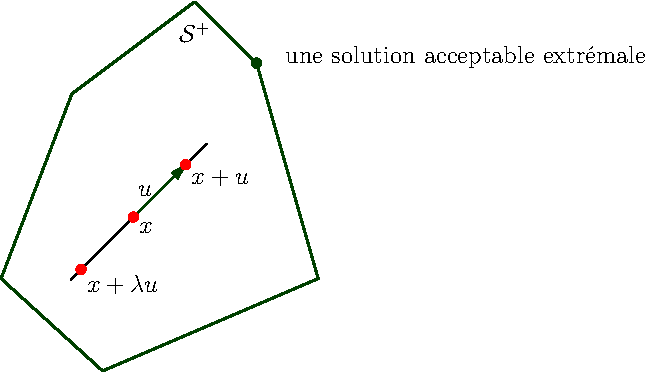
\includegraphics[width=7cm]{Eproglin_1.pdf}
  % Eproglin_1.pdf: 340x3 px, 72dpi, 11.99x0.11 cm, bb=0 0 340 3
  \caption{\'Etude locale}
  \label{fig: Eproglin_1}
\end{figure}
\noindent
On note $I(x,u) = \left\lbrace \lambda \in \R \text{ tq } x + \lambda u \in \mathcal{S}^+ \right\rbrace$ et
\[
  \begin{aligned}
    &m^+(x,u) = \min\left\lbrace \frac{x_j}{u_j}, j \in J^+(u)\right\rbrace &\text{ si } J^+(u) \neq \emptyset,\\
    &m^-(x,u) = \min\left\lbrace \frac{x_j}{|u_j|}, j \in J^-(u)\right\rbrace &\text{ si } J^-(u) \neq \emptyset.
  \end{aligned}
\]
Il est utile de remarquer que 
\[
  \begin{aligned}
    &J^-(x) = \emptyset,\; J(x) = J^+(x) \neq \emptyset \text{ car } x\in \mathcal{S}^+ \text{(donc non nul)}, \\
    &J(u) = J^-(u) \cup J^+(u) \neq \emptyset \text{ car $u$ non nul}.
  \end{aligned}
\]

\begin{enumerate}
  \item Montrer que 
\[
  \begin{aligned}
    &m^+(x,u) \geq 0, &m^+(x,u) > 0 \Leftrightarrow J^+(u)  \subset J(x), \\ 
    &m^-(x,u) \geq 0, &m^-(x,u) > 0 \Leftrightarrow J^-(u)  \subset J(x).
  \end{aligned}
\]

  \item Montrer que $x + \lambda u \in \mathcal{S}$ pour tout $\lambda \in \R$.
  \item 
  \begin{enumerate}
    \item Montrer que 
\[
  I(x,u) =
  \left\lbrace
  \begin{aligned}
    &\left[ -m^+(x,u), m^-(x,u)\right] &\text{ si }& J^+(u)\neq \emptyset \text{ et } J^-(u)\neq \emptyset \\
    &\left[ -m^+(x,u), +\infty\right[ &\text{ si }&  J^-(u) = \emptyset \\
    &\left] -\infty, m^-(x,u)\right] &\text{ si }& J^+(u) = \emptyset 
  \end{aligned}
  \right. .
\]
    \item Montrer que 
\[
  \left( \min I(x,u) = 0 \text{ ou } \max I(x,u) = 0\right)
  \Leftrightarrow
  \exists j \in \llbracket 1,n \rrbracket \text{ tq } \left( u_j \neq 0 \text{ et } x_j = 0\right).
\]

         \end{enumerate}
\end{enumerate}
On dit que $x \in \mathcal{S}^+$ est une solution \emph{extrémale} si et seulement si
\[
  \forall u \in S\setminus \left\lbrace 0_{\R^n} \right\rbrace,\; \left( \min I(x,u) = 0 \text{ ou } \max I(x,u) = 0 \right). 
\]
Géométriquement, on peut se convaincre qu'une solution acceptable extrémale correspond à un \og coin\fg~ sur la figure \ref{fig: Eproglin_1}. La partie suivante propose une caractérisation algébrique.
\clearpage

\subsection*{Partie 3. Noyau et relations entre colonnes}
\begin{enumerate}
  \item
  \begin{enumerate}
    \item Soit $u$ non nul dans $S$. Montrer que la famille $\left( v_j, j\in J(u)\right)$ est liée.
    \item Soit $J$ une partie de $\llbracket 1,n \rrbracket$ telle que $\left( v_j, j\in J\right)$ liée. Montrer qu'il existe $u$ non nul dans $S$ avec $J(u) \subset J$.
  \end{enumerate}

  \item Caractérisation de l'extrémalité.  Soit $x \in \mathcal{S}^+$ une solution acceptable.
  \begin{enumerate}
    \item Soit $u$ non nul dans $S$. Montrer que 
\[
  \left(\min I(x,u) = 0\text{ ou } \max I(x,u)=0 \right) \text{ FAUX }
  \Leftrightarrow
  \overline{J(x)} \subset \overline{J(u)}.
\]
    \item Montrer que 
\[
  x \text{ non extrémale } \Leftrightarrow S \cap \Vect(e_j,\, j \in J(x)) \neq \left\lbrace 0_{\R^n} \right\rbrace
  \Leftrightarrow \left(v_j, j\in J(x)\right) \text{ liée}.
\]
    \item En déduire 
\[
  x \text{ extrémale } \Leftrightarrow \left(v_j, j\in J(x)\right) \text{ libre}.
\]
  \end{enumerate}
  \item Soit $x \in \mathcal{S}^+$ extrémale. 
  Montrer qu'il existe $J \subset \llbracket 1,n \rrbracket$ telle que $J(x) \subset J$ avec  
  $\mathcal{B} = \left( v_j, j\in J\right)$ base de $\mathcal{M}_{m 1}(\R)$. \footnote{Attention, si $n(x) < m$, il peut exister plusieurs parties $J$ vérifiant ces conditions.}
\end{enumerate}
\clearpage

\subsection*{Partie 4. Algorithme du simplexe}
\begin{enumerate}
  \item Soit $x \in \mathcal{S}^+$ non extrémale. On veut montrer
\[
\exists y \in \mathcal{S}^+ \text{ telle que } J(y) \subsetneq J(x) \text{ et } \gamma(y) \leq \gamma(x).
\]
  \begin{enumerate}
    \item Montrer que 
\[
  \exists j\in J(x), \exists u =(u_1, \cdots,u_n) \in S \text{ non nul tels que } J(u) \subset J(x) \text{ et } u_j = 1.
\]
    \item Montrer que $m^+(x,u) > 0$. Montrer que $J^-(u) \neq \emptyset$ entraine $m^-(x,u) > 0$. Montrer que $J^-(u) = \emptyset$ entraine $\gamma(u) \geq 0$.
    \item Conclure en considérant $I(x,u)$.
  \end{enumerate}
 
  \item D'un extrème à l'autre.\newline
Soit $x \in \mathcal{S}^+$ extrémale avec $J \subset \llbracket 1,n \rrbracket$ telle que 
\[
  J(x) \subset J \text{ et } \mathcal{B} = \left( v_j, j\in J\right) \text{ base de } \mathcal{M}_{m 1}(\R).
\] 
Soit $k \in \llbracket 1,n \rrbracket,\, k \notin J$. On définit $u = (u_1, \cdots, u_n) \in \R^n$ par :
\[
\left\lbrace
  \begin{aligned}
    &u_l = 0 &\text{ si }& l \notin J \cup \left\lbrace k\right\rbrace\\
    &u_k = 1 & & \\
    &u_j = - \text{ coordonnée de $v_k$ relative à } v_j \text{ dans } \mathcal{B} &\text{ si }& j \in J
  \end{aligned}
\right. .
\]
  \begin{enumerate}
    \item Montrer que $u$ est un élément non nul de $S$.
    \item Montrer que 
\[
  J(u) \subset J(x) \cup \left\lbrace k\right\rbrace, \hspace{0.4cm}
  J^+(u) \neq \emptyset \text{ et } m^+(x,u) = 0, \hspace{0.4cm}
  m^-(x,u) > 0 \text{ on le note $\theta$}.
\]
    \item On pose $y = x + \theta u$. Montrer que $y$ est une solution acceptable extrémale. 
   \end{enumerate}
  
  \item Variation du coût. On garde les conditions et notations de la question précédente.\newline
Montrer que $\gamma(y) < \gamma(x) \Leftrightarrow \gamma(u) < 0$.
 
   \item Optimalité. On garde les conditions et notations de la question 3.\newline
   Pour chaque $k \notin J$, comme le $u \in S$ dépend de $k$, on le note $s_k$.
   \begin{enumerate}
     \item Montrer que $\left(s_k , k \in \overline{J}\right)$ est une base de $S$. Quelles sont les coordonnées de $u=(u_1, \cdots,u_n)\in S$ dans cette base?
     \item On suppose que $\gamma(s_k)\geq 0$ pour tous les $k \in \overline{J}$. Montrer que 
     \[
       \forall y \in \mathcal{S}^+, \; \gamma(x) \leq \gamma(y).
     \]
   \end{enumerate}
  \item Présenter le principe de l'algorithme du simplexe permettant de calculer un $x\in \mathcal{S}^+$ tel que 
\[
  \gamma(x) = \min\left\lbrace \gamma(y),\; y \in \mathcal{S}^+ \right\rbrace.
\]
  On s'attachera à justifier la terminaison de l'algorithme.
\end{enumerate}

